\documentclass[12pt, a4paper, oneside]{report}
\usepackage[utf8]{inputenc}
% \usepackage{CormorantGaramond}
\usepackage{hyperref}
\usepackage{graphicx}
\graphicspath{ {./docs/} }

\hypersetup{
	colorlinks=true,
	linkcolor=black,
	filecolor=blue,
	urlcolor=black,
	pdftitle={Report on S6 project},
}

\title{\textbf{Report on the ConnAIct 4 project}}
\author{\normalsize François Barnouin, Cindy Do, Henri Gasc\\\normalsize Hamza Jad Al Aoun, Guillaume Ung\\\\\\\\\\\\\\\\\\Under the supervision of \textbf{\textit{Nicholas Evans}}}
\date{}

\begin{document}
	\maketitle
	\tableofcontents

	\chapter{Introduction}
	The Connect 4 game is a classical and well-known game. It is often used as a mean to evaluate how comfortable someone is in it's programming capabilities. \\
	Today, we are the one evaluated on it, but with a few twists. We have to create an AI to play the game, communicate with another player wirelessly, and accept inputs as signs that someone does to a camera. \\
	This represents a four-way challenge.
	\begin{itemize}
		\item First, we have to code the logic behind the Connect 4 in a way that makes it easy for the other part to work with.
		\item Second, our AI need to be fast, robust, and precise.\footnote{More on those terms in the dedicated section (\ref{AI_section}).} (change them if needed)
		\item Thirdly, we have to choose some gestures, make it fast and easy to use.
		\item Last but not least, we need to define the protocols and technologies used to communicate.
	\end{itemize}

	\chapter{User manual}

	\section{Specifications}
	To use the whole project (meaning, with the camera, the AI in C++, the communication module), you need to have installed:
	\begin{itemize}
		\item A version of Python (preferably >= 3.11),
		\item A C++ compiler (\textit{clang++} produce better binary but \textit{g++} works too),
		\item A working bash interpreter,
		\item A Raspberry Pi with a camera module, a Bluetooth chip, and at least 2 GB of RAM. make sure the code works on raspbian 32 bits
	\end{itemize}
	All those requirements are easy to fulfil, and you should not have anything to install on your own. \\

	\section{Setting up}
	When the previous requirements are fulfilled, you only need to use the \textit{launch.sh} script, and every other software and libraries required should be installed. \\
	If the script does not find something, then it prints it and launches the program with some options disabled.

	\section{Indications}
	When the program open, you should be able to understand easily what to do, and how to do it. However, if it is needed, here is the explanation about the different screens of the game. \\

	This first screen presents you with the menu. You may go to the options or play menu. \\
	\hspace*{1cm} In the options screen, you can choose the language you want the program to use, if you want to use the camera, if you want to have sound when playing. To change those, just click on the relevant icon. \\
	\hspace*{1cm} The play menu let you choose if you want to play against a human, against an AI, or if you want to watch two AI battle each other for domination. When choosing a game including an AI, you will be able to select its difficulty. \\

	When playing, you can use your mouse or you hand (if you activated the camera) to select the column in which you want to put your token in. The selected column will be highlighted.

	\chapter{Technical manual}
	% A technical manual that explains:
	% \begin{itemize}
	% 	\item The design and development choices, motivates them, and optionally compares them with other possible choices.
	% 	\item The software architecture and the role of each file in the source code archive.
	% 	\item How the produced source code has been validated and verified, and with what results.
	% 	\item What difficulties have been encountered and how they have been solved.
	% \end{itemize}

	\section{Interface}
	For the interface, we chose to use Python for its ease of use. We used classes because this representation is very flexible and close to what we want. \\

	Each “screen” of the game (All the menus + the game screen (with the board)) is its own class, inherited from a base class common to all screens. The basic principle to display things is the same, only the content is different. This way, a graphical continuity is preserved between all screens. \\

	Classes are made for each player, the board of the game, the gestures, the AI, and the communication, as well as for the game itself. \\
	This way, all the code is well compartmented and we can easily change how something is done in the backend as long as we don't change the API (meaning, the arguments and return statements of the functions) calls. \\

	The most challenging part in writing the interface was managing to integrate the communication, AI, and gestures recognition in the code in a way that makes it easy to modify things. Using classes was a way to solve those problems before they became hindrances.

	\section{AI}\label{AI_section}

	We went through several stages while implementing the artificial intelligence. We improved the code step-by-step in order to have the best behaviour possible. \\

	\subsection{First stage}
	The first stage was very simple, we had to implement some basic functions. \\
	We decided to represent the state of a game using 64 bits numbers. This representation is called a bitboard. The presence of a token in a position is translated into a 1 in its place on the bitboard. \\
	We use an 8 by 8 board, with the top row and right-most column always empty.

	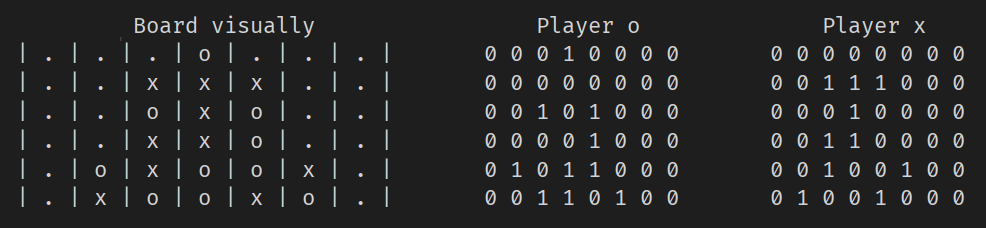
\includegraphics[scale=0.35]{example.png} \\

	Then, we implemented functions In order to drop a piece in a column and another to scan the board in order to see if a player had won the game. At this point, by simply displaying the board, it was possible to play connect 4 with two human players. That’s a start but we are not quite finished yet. \\

Second stage, implementation of a basic AI which to not foresee possibilities in the future:
	We first needed to give the computer some indication so it can understand in which column he had to play. This is the start of our first heuristic function (or evaluation function): this is the scoring function that determines the score of a given state by using specific features of the state of the game. The specific features mentioned here were obviously the number of tokens that were aligned in each direction (horizontally, vertically and diagonally). We created a scanning function. It created a window of four emplacements of the board and it counted the number of player 1’s tokens, player 2’s tokens and the number of available emplacements. We then gave points to the columns according to the number of two in a rows and three in a row the column. Which means the more points a column had, the more likely future possibilities could be created. Of course, the heuristic is designed in a way that if a player can win or defend from the opponent’s three in a row, it will automatically do it.
	This first artificial intelligence was simple, could win against player choosing a column randomly or even against very distracted players (we did lose ashamedly a couple of times). However there was no strategy at all, we could not settle for that. We had to go further. \\

Third stage, implementation of the minimax algorithm.
	First, we decided to implement a decision tree. It is a tree structure, where each internal node denotes a test on an attribute, each branch represents an outcome of the test, and each leaf node (terminal node) holds a class label. It is especially useful in logic games such as the connect 4 since it shows all the possible choices. The game includes 7 branches each time (except when a column is full or when the game ends). After the move of the first player, the second one choose a column out of seven, continuing from the other player’s choice of the decision tree.
	Alright so now we have created a structure in which the state of the future boards will be represented. Now we have to choose the method in order to move around in this structure and choose the best path possible each time. For that, we used the minimax algorithm. It is a recursive algorithm which is used in decision-making and game theory especially in AI game. It tries to analyze the possible paths and returns the optimal move for a player assuming that a player is also playing optimally. In order to accomplish that, there is a maximizing player (with which we try to have as many points as possible, using the same heuristic function) and a minimizing player (with which we try to have as less points as possible). The algorithm performs a depth-first search (DFS), it will explore the complete game tree as deep as possible, all the way down to the leaf nodes.
The minimax was not hard to implement, and after this stage we had  decent AI. However the computational time was way too long, so we had to implement other features and optimizations of our code. \\

Fourth stage, features and optimizations:
	First, we implemented alpha-beta pruning. It introduces a score window [alpha, beta] within which you search the actual score of the game’s state. Hence, we do not have to explore paths and compute  additionally scores associated with boards that are not better than an already calculated score and the column linked to the path related. There are 3 possible cases :  \\

	\hspace*{1cm} If the actual score of the position is within the range, then the alpha-beta function should return the exact score.
	\hspace*{1cm} If the actual score of the position is lower than alpha, then the alpha-beta function is allowed to return any upper bound of the actual score that is lower or equal to alpha.
	\hspace*{1cm} If the actual score of the position greater than beta, then the alpha-beta function is allowed to return any lower bound of the actual score that is greater or equal to beta \\

Thus, the exploration of the tree is narrowed , we are able to prune the search tree as soon as we have a computed score greater than beta.

	Then, several other optimizations were made: we translated in C++ the minimax algorithm to reduce the computing time, we made the algorithm explore the columns starting in the middle and expanding one by one to the sides because there are more possibilities to win by playing in the middle. 
	Since Connect 4 is a zero sum game, we also decided to use a variant form of the minimax : the Negamax. It simplified the search algorithm: instead of using two separate subroutines for the Minimizing player and the Maximizing player, the value of player 1 is the negation of the value of player 2. Thus, a single procedure can be used to evaluate the board’s state of both players.
	Several other small computing time related optimizations were made. In order to judge those optimisations several benchmarks were made.


Finally, our artificial intelligence was made, and the deeper the level, the harder it was for us to beat it. The only time when losing gives a truly satisfying result ! But how could we judge the efficiency of our artificial intelligence ? We decided to create a small set of the following criteria to do so: \\

\hspace*{1cm} An AI at any depth must always beat a player that is always choosing a column randomly.
\hspace*{1cm} An AI at any depth must beat an AI which is at a depth level strictly lower than itself.
\hspace*{1cm} For a given depth level, the AI who starts first must beat an AI at the same depth level.\\

Those criteria were evaluated and reported in the following graph (insert graph and comment results) \\


	\section{Gestures}

	\section{Communication}

	\chapter{Conclusion}
\end{document}
